\section{Assembling the linear system of equations}
\label{Sec1:assembly}
In the previous section, $6M$ equations for the $6M$ unknowns $A_{m,n}^{(i)}$, $B_{m,n}^{(i)}$ and $C_{m,n}^{(i)}$ for all $n>0$ and $4M$ equations for the $4M$ unknowns for $n = 0$ was established. So far, the solution has been presented for $M$ elastic spherical shells with standard displacement and pressure conditions; \textit{the default case with Neumann-to-Neumann conditions}. By some matrix manipulations of the global matrix, one can implement other cases as well, including solid spheres, and single Neumann conditions replacing the Neumann-to-Neumann conditions on the innermost domain.

\subsection{The default case with Neumann-to-Neumann conditions}
For the default case all equations can be collected into one single linear system of equations 
\begin{equation}\label{Eq1:SystemOfEquations}
	\vec{H}_n \vec{C}_n = \vec{D}_n
\end{equation}
where\footnote{Note that the matrix pattern is scaled for the case $n>0$, as $\vec{H}_{m,n}^{(1)}\in\R^{4\times 4}$ and $\vec{H}_{m,n}^{(4,j)}\in\R^{1\times 4}$ for $n>0$, as opposed to $\vec{H}_{m,n}^{(1)}\in\R^{2\times 2}$ and $\vec{H}_{m,n}^{(4,j)}\in\R^{1\times 2}$ when $n=0$ (for $j = 1, 2$).}
\begin{equation*}\resizebox{\textwidth}{!}{$
	\vec{H}_n = \left[
	\begin{BMAT}(rc){c.c.c.c.c.c.c}{c.c.c.c.c.c.c.c.c}
	\begin{BMAT}(b){c}{c}H_{1,1,n}^{(3,0)}\end{BMAT} & {\hskip2.3em\relax}\vec{H}_{1,n}^{(4,0)}{\hskip2.3em\relax} & {\hskip4em\relax} & {\hskip2.3em\relax}\phantom{\vec{H}_{1,n}^{(4,0)}}{\hskip2.3em\relax}  & {\hskip4em\relax} & {\hskip2.3em\relax}\phantom{\vec{H}_{1,n}^{(4,0)}}{\hskip2.3em\relax}& \\
	\begin{BMAT}(rc){c}{c.ccc}H_{1,1,n}^{(2,0)}\\ \phantom{H_{1,n}^{(2,0)}}\\ \phantom{H_{1,n}^{(2,0)}}\\ \phantom{H_{1,n}^{(2,0)}}\end{BMAT} & \vec{H}_{1,n}^{(1)} & \begin{BMAT}(rc){c}{ccc.c} \phantom{H_{2,n}^{(2,0)}}\\ \phantom{H_{2,n}^{(2,0)}}\\ \phantom{H_{2,n}^{(2,0)}}\\ {\hskip0.5em\relax}\vec{H}_{2,n}^{(2,1)}{\hskip0.5em\relax}\end{BMAT} & & & &\\
	 & \vec{H}_{1,n}^{(4,1)} & \vec{H}_{2,n}^{(3,1)} & & & &\\
	 & & \vec{H}_{2,n}^{(3,0)} & \vec{H}_{2,n}^{(4,0)} & & &\\
	 & & \begin{BMAT}(rc){c}{c.ccc}{\hskip0.5em\relax}\vec{H}_{2,n}^{(2,0)}{\hskip0.5em\relax}\\ \phantom{H_{1,n}^{(2,0)}}\\ \phantom{H_{1,n}^{(2,0)}}\\ \phantom{H_{2,n}^{(2,0)}}\end{BMAT} & \ddots & \begin{BMAT}(rc){c}{ccc.c} \phantom{H_{1,n}^{(2,0)}}\\ \phantom{H_{1,n}^{(2,0)}}\\ \phantom{H_{1,n}^{(2,0)}}\\ {\hskip0.5em\relax}\vec{H}_{M,n}^{(2,1)}{\hskip0.5em\relax}\end{BMAT} & &\\
	 & & & \vec{H}_{M-1,n}^{(4,1)} & \vec{H}_{M,n}^{(3,1)} & &\\
	 & & & & \vec{H}_{M,n}^{(3,0)} & \vec{H}_{M,n}^{(4,0)} &\\
	 & & & & \begin{BMAT}(rc){c}{c.ccc}{\hskip0.5em\relax}\vec{H}_{M,n}^{(2,0)}{\hskip0.5em\relax}\\ \phantom{H_{1,n}^{(2,0)}}\\ \phantom{H_{1,n}^{(2,0)}}\\ \phantom{H_{1,n}^{(2,0)}}\end{BMAT} & \vec{H}_{M,n}^{(1)} & \begin{BMAT}(rc){c}{ccc.c} \phantom{H_{1,n}^{(2,0)}}\\ \phantom{H_{1,n}^{(2,0)}}\\ \phantom{H_{1,n}^{(2,0)}}\\ H_{1,M+1,n}^{(2,1)}\end{BMAT}\\
	 & & & & & \vec{H}_{M,n}^{(4,1)} & H_{1,M+1,n}^{(3,1)}
	\end{BMAT} 
	\right]$}
\end{equation*}
with submatrices $\vec{H}_{m,n}^{(1)}$ has entries given in \Cref{Eq1:K1n} and \Cref{Eq1:K10}. The submatrices 
\begin{equation*}
	\vec{H}_{m,n}^{(2,j)} = \begin{bmatrix}
		H_{1,m,n}^{(2,j)} & H_{2,m,n}^{(2,j)}
	\end{bmatrix}
\end{equation*}
has entries given in \Cref{Eq1:K2}. The submatrices
\begin{equation*}
	\vec{H}_{m,n}^{(3,j)} = \begin{bmatrix}
		H_{1,m,n}^{(3,j)} & H_{2,m,n}^{(3,j)}
	\end{bmatrix}
\end{equation*}
has entries given in \Cref{Eq1:K3}. The submatrices
\begin{equation*}
	\vec{H}_{m,n}^{(4,j)} = \begin{bmatrix}
		H_{1,m,n}^{(4,j)} & H_{2,m,n}^{(4,j)} & H_{3,m,n}^{(4,j)} & H_{4,m,n}^{(4,j)}
	\end{bmatrix}
\end{equation*}
for $n>0$, and 
\begin{equation*}
	\vec{H}_{m,n}^{(4,j)} = \begin{bmatrix}
		H_{1,m,n}^{(4,j)} & H_{2,m,n}^{(4,j)}
	\end{bmatrix}
\end{equation*}
for $n=0$, has entries given in \Cref{Eq1:K4}. The entries $H_{1,1,n}^{(3,0)}$, $H_{1,1,n}^{(2,0)}$, $H_{1,M+1,n}^{(3,1)}$ and $H_{1,M+1,n}^{(2,1)}$, are given in \Cref{Eq1:K3011,Eq1:K2011,Eq1:K311Mp1,Eq1:K211Mp1}, respectively.

Finally, the collumn vectors in~\Cref{Eq1:SystemOfEquations} are given by
\begin{equation*}\resizebox{\textwidth}{!}{$
	\vec{C}_n = \begin{bmatrix}
		C_{1,n}^{(1)}\\
		\vec{A}_{1,n}\\
		\vec{B}_{1,n}\\
		\vec{C}_{2,n}\\
		\vdots\\
		\vec{A}_{M-1,n}\\
		\vec{B}_{M-1,n}\\
		\vec{C}_{M,n}\\
		\vec{A}_{M,n}\\
		\vec{B}_{M,n}\\
		C_{M+1,n}^{(1)}
	\end{bmatrix}\quad
	\vec{A}_{m,n} = \begin{bmatrix}
		A_{m,n}^{(1)}\\
		A_{m,n}^{(2)}\\
	\end{bmatrix}\quad
	\vec{B}_{m,n} = \begin{bmatrix}
		B_{m,n}^{(1)}\\
		B_{m,n}^{(2)}\\
	\end{bmatrix}\quad
	\vec{C}_{m,n} = \begin{bmatrix}
		C_{m,n}^{(1)}\\
		C_{m,n}^{(2)}\\
	\end{bmatrix}\quad
	\vec{D}_n = \begin{bmatrix}
		D_{1,n}\\
		D_{2,n}\\
		0\\
		0\\
		\vdots\\
		0
	\end{bmatrix}.$}
\end{equation*} 
where the entries $D_{1,n}$ and $D_{2,n}$, are given in \Cref{Eq1:D1,Eq1:D2}, respectively.

\subsection{Alternative boundary conditions}
\label{Subsec1:alternativeBoundaryConditions}
By removing the last five (three) rows and columns of $\vec{H}_n$ for $n>0$ ($n=0$), the Neumann-to-Neumann boundary condition (NNBC) is replaced by a single Neumann condition\footnote{That is, the normal velocity component of the fluid at the surface is zero, such that $u_{\mathrm{r}}=0$ in \Cref{Eq1:firstBC}. This is often referred to as a sound-hard boundary condition, SHBC.}
\begin{equation}
	\pderiv{p_{\mathrm{tot},M}}{r} = 0
\end{equation}
at the innermost solid domain. This Neumann boundary condition may be replaced by other boundary conditions, for example the Robin boundary condition (impedance boundary condition) by corresponding manipulation of the matrix $\vec{H}_n$. By removing the last row and column of the matrix $\vec{H}_n$ a Neumann condition ($\sigma_{\mathrm{rr}}=0$) is obtained on the inside of the innermost shell\footnote{This is often referred to as a sound-soft boundary condition, SSBC.}.  Moreover, one can model scattering on solid spheres\footnote{This type of boundary conditions is named elastic sphere boundary conditions, ESBC.} (such that the innermost domain is no longer fluid, but solid) by removing the three last rows (corresponding to the boundary conditions at $R_{1,M}$) and three columns (corresponding to the coefficients $A_{M,n}^{(2)}$, $B_{M,n}^{(2)}$ and $C_{M+1,n}^{(1)}$) of the matrix $\vec{H}_n$ (and corresponding entries of $\vec{C}_n$ and $\vec{D}_n$). The reason for not using the coefficients $A_{M,n}^{(2)}$ and $B_{M,n}^{(2)}$ is that the corresponding spherical Bessel functions of second kind are unbounded at the origin, such that these coefficients must be set to zero. The displacement of the inner solid sphere is then given by
\begin{equation}
	\vec{u}_M = u_{\mathrm{r},M} \vec{e}_{\mathrm{r}} + u_{\upvartheta,M} \vec{e}_\upvartheta
\end{equation}
where
\begin{align}
	u_{\mathrm{r},M}(r,\vartheta) &= \frac{1}{r}\sum_{n=0}^\infty Q_n^{(0)}(\vartheta)\left[A_{M,n}^{(1)}S_{1,n}^{(1)}(a_M r)+B_{M,n}^{(1)}T_{1,n}^{(1)}(b_M r)\right]\\
	u_{\upvartheta,M}(r,\vartheta) &= \frac{1}{r}\sum_{n=0}^\infty Q_n^{(1)}(\vartheta)\left[A_{M,n}^{(1)}S_{2,n}^{(1)}(a_M r)+B_{M,n}^{(1)}T_{2,n}^{(1)}(b_M r)\right].
\end{align} 
It should be noted that the solution is well defined also at the origin due to the formulas in \Cref{Eq1:BesselLimits,Eq1:BesselLimits2}. In fact, on can show that (using \Cref{Eq1:SphericalToXfun})
\begin{equation*}
	\lim_{r\to 0}\vec{u}_M(r,\vartheta) = \frac13 \left[a_MA_{M,1}^{(1)}-2b_MB_{M,1}^{(1)}\right]\vec{e}_3,
\end{equation*}
and (using \Cref{Eq1:SphericalToXJacobian})
\begin{align*}
	\lim_{r\to 0}\pderiv{u_{1,M}}{x_1}(r,\vartheta) &= \frac{G_M}{9K_M}\left(4a_M^2-3b_M^2\right)A_{M,0}^{(1)} - \frac{1}{15}\left(a_M^2 A_{M,2}^{(1)} - 3b_M^2B_{M,2}^{(1)}\right)\\
	\lim_{r\to 0}\pderiv{u_{2,M}}{x_2}(r,\vartheta) &= \frac{G_M}{9K_M}\left(4a_M^2-3b_M^2\right)A_{M,0}^{(1)} - \frac{1}{15}\left(a_M^2 A_{M,2}^{(1)} - 3b_M^2B_{M,2}^{(1)}\right)\\
	\lim_{r\to 0}\pderiv{u_{3,M}}{x_3}(r,\vartheta) &= \frac{G_M}{9K_M}\left(4a_M^2-3b_M^2\right)A_{M,0}^{(1)} + \frac{2}{15}\left(a_M^2 A_{M,2}^{(1)} - 3b_M^2B_{M,2}^{(1)}\right)\\
	\lim_{r\to 0}\pderiv{u_{i,M}}{x_j}(r,\vartheta) &= 0\quad\text{for}\quad i\neq j
\end{align*}
where $u_{i,M}$ is the $i^{\mathrm{th}}$ Cartesian component of $\vec{u}$. The stress field can then be computed in the origin as (using \Cref{Eq1:StressTransformFromCartToSpherical})
\begin{align*}
	\lim_{r\to 0}\sigma_{11,M}(r,\vartheta) &= \frac{G_M}{15}\left[5\left(4a_M^2-3b_M^2\right)A_{M,0}^{(1)} - 2a_M^2A_{M,2}^{(1)} +6b_M^2B_{M,2}^{(1)}\right]\\
	\lim_{r\to 0}\sigma_{22,M}(r,\vartheta) &= \frac{G_M}{15}\left[5\left(4a_M^2-3b_M^2\right)A_{M,0}^{(1)} - 2a_M^2A_{M,2}^{(1)} +6b_M^2B_{M,2}^{(1)}\right]\\
	\lim_{r\to 0}\sigma_{33,M}(r,\vartheta) &= \frac{G_M}{15}\left[5\left(4a_M^2-3b_M^2\right)A_{M,0}^{(1)} + 4a_M^2A_{M,2}^{(1)} -12b_M^2B_{M,2}^{(1)}\right]\\
	\lim_{r\to 0}\sigma_{23,M}(r,\vartheta) &= 0\\
	\lim_{r\to 0}\sigma_{13,M}(r,\vartheta) &= 0\\
	\lim_{r\to 0}\sigma_{12,M}(r,\vartheta) &= 0
\end{align*}
where $\sigma_{ij,M}$ is the stress field in the solid sphere in Cartesian coordinates. If the innermost domain is a fluid, then
\begin{align*}
	\lim_{r\to 0}p_{M+1}(r,\vartheta) &= C_{M+1,0}^{(1)}\\
	\lim_{r\to 0}\nabla p_{M+1}(r,\vartheta) &= \frac{k_{M+1}}{3}C_{M+1,1}^{(1)} \vec{e}_3\\
	\lim_{r\to 0}\nabla^2 p_{M+1}(r,\vartheta) &= -k_{M+1}^2 C_{M+1,0}^{(1)}.
\end{align*}
Finally, note that one can model connected fluid or solid layers by manipulating the the matrix $\vec{H}_n$ to match the pressure and displacement condition between these domains. An example of such an application is air bubbles in water~\cite{Fender1972sfa}.

\subsection{Summary of solution formulas}
In this sub section, the final expressions have been summarized (see \Cref{Fig1:function_distribution}).
\begin{figure}
	\centering
	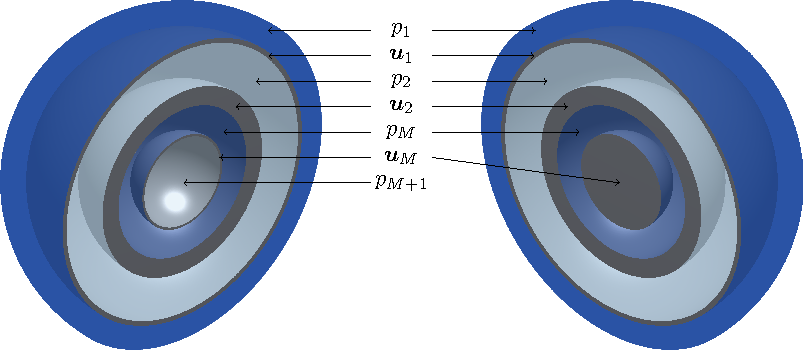
\includegraphics{../../LaTeX/createFigures/TikzFigures/article_e3Dss_PhD/function_distribution}
%	\includegraphics[scale=1]{\graphicsFolder/Figure3}
	\caption{Illustration (clip view) of a model (to the left) with 3 steel shells and a model (to the right) with 2 steel shells surrounding a solid steel sphere, illustrating the distribution of functions (in the case $M=3$). The model to the left models a fluid as the innermost domain, while the model to the right models a solid domain as the innermost domain (note that the expression $\vec{u}_M$ is slightly altered in this case).}
	\label{Fig1:function_distribution}
\end{figure}
Recall that $\hankel_n^{(i)}$, $Z_{j,n}^{(i)}$, $S_{j,n}^{(i)}$ and $T_{j,n}^{(i)}$ are all derived from spherical Bessel functions ($\besselj_n$ and $\bessely_n$), while $Q_n^{(i)}$ are derived from Legendre functions. All coefficients ($A_{m,n}^{(i)}$, $B_{m,n}^{(i)}$ and $C_{m,n}^{(i)}$) are found by solving the linear system of equations in \Cref{Eq1:SystemOfEquations}. The scattered pressure field in the outermost (unbounded) fluid domain, the $m^{\mathrm{th}}$ fluid layer (for $2\leq m \leq M$), and the innermost fluid domain (if present), are given by
\begin{align}\label{Eq1:Summary_p1}
p_1(r,\vartheta) &= \sum_{n=0}^\infty Q_n^{(0)}(\vartheta) C_{1,n}^{(1)} \hankel^{(1)}_n(k_1 r)\\\label{Eq1:Summary_pm}
p_m(r,\vartheta) &= \sum_{n=0}^\infty Q_n^{(0)}(\vartheta)C_{m,n}^{(i)} Z_n^{(i)}(k_m r)\\
	p_{M+1}(r,\vartheta) &= \sum_{n=0}^\infty Q_n^{(0)}(\vartheta) C_{M+1,n}^{(1)} \besselj_n(k_{M+1} r),\label{Eq1:Summary_pM1}
\end{align}
respectively. The displacement field in the $m^{\mathrm{th}}$ solid domain is given by
\begin{equation}
	\vec{u}_m = u_{\mathrm{r},m} \vec{e}_{\mathrm{r}} + u_{\upvartheta,m} \vec{e}_\upvartheta\label{Eq1:Summary_u}
\end{equation}
where
\begin{align}
	u_{\mathrm{r},m}(r,\vartheta) &= \frac{1}{r}\sum_{n=0}^\infty Q_n^{(0)}(\vartheta)\left[A_{m,n}^{(i)}S_{1,n}^{(i)}(a_m r)+B_{m,n}^{(i)}T_{1,n}^{(i)}(b_m r)\right]\\
	u_{\upvartheta,m}(r,\vartheta) &= \frac{1}{r}\sum_{n=0}^\infty Q_n^{(1)}(\vartheta)\left[A_{m,n}^{(i)}S_{2,n}^{(i)}(a_m r)+B_{m,n}^{(i)}T_{2,n}^{(i)}(b_m r)\right].
\end{align} 
If the inner domain is a solid domain, the terms involving $S_{1,n}^{(2)}$ and $T_{1,n}^{(2)}$ in $\vec{u}_M$, are not present.